\section{Appendix: Project Management}
\label{app:screen}

This chapter presents a detailed examination of the project management approaches used for this research. It begins with an overview of the project management plan, followed by a Gantt chart illustrating the project timeline and concludes with a risk analysis.
This section provides an overview of the project management techniques and planning strategies adopted to ensure the successful completion of this research project, scheduled from September 2024 to May 2025. \\
Effective project management is necessary to structure various phases of the research including model development and documentation within a limited timeframe. The plan is carefully designed to accommodate potential challenges faced during the course of the project. Hence, it enables flexibility throughout the project. 
\vspace{-3 cm}
\subsection{Overview of Project Management Approach} \leavevmode
\vspace{-0.2 cm}
\\This research project uses an individual Agile approach, focusing on flexibility, iterative development, and continuous improvement. Agile and Scrum methodologies are used for team-based projects and individual research projects. \\The project is divided into sprints, each with a review phase to evaluate progress and assess challenges. This structured yet flexible management style supports continuous improvement and responsiveness to new findings. Agile methodologies are particularly beneficial in healthcare research, where data complexity and critical outcomes demand a flexible approach. Agile methodologies are being widely used across various industries such as financial services, energy, healthcare, pharmaceuticals, and education \cite{zaidi2024review}.
\vspace{-3 cm}
\subsection{Project Plan}\leavevmode
\vspace{-0.2 cm}
\\ A Gantt Chart is a tool suggested by Agile project management. It is used for tracking the project’s progress during its timeline. \hyperref[fig:Gantt Chart]{Figure 2} below shows the Gantt chart demonstrating the stages of development of the project. Big tasks have been broken down into smaller sub-tasks for easier implementation. Dependencies between tasks have been added. A buffer period has been allocated to each task to ensure its timely completion.

\begin{figure}[H]
    \centering
    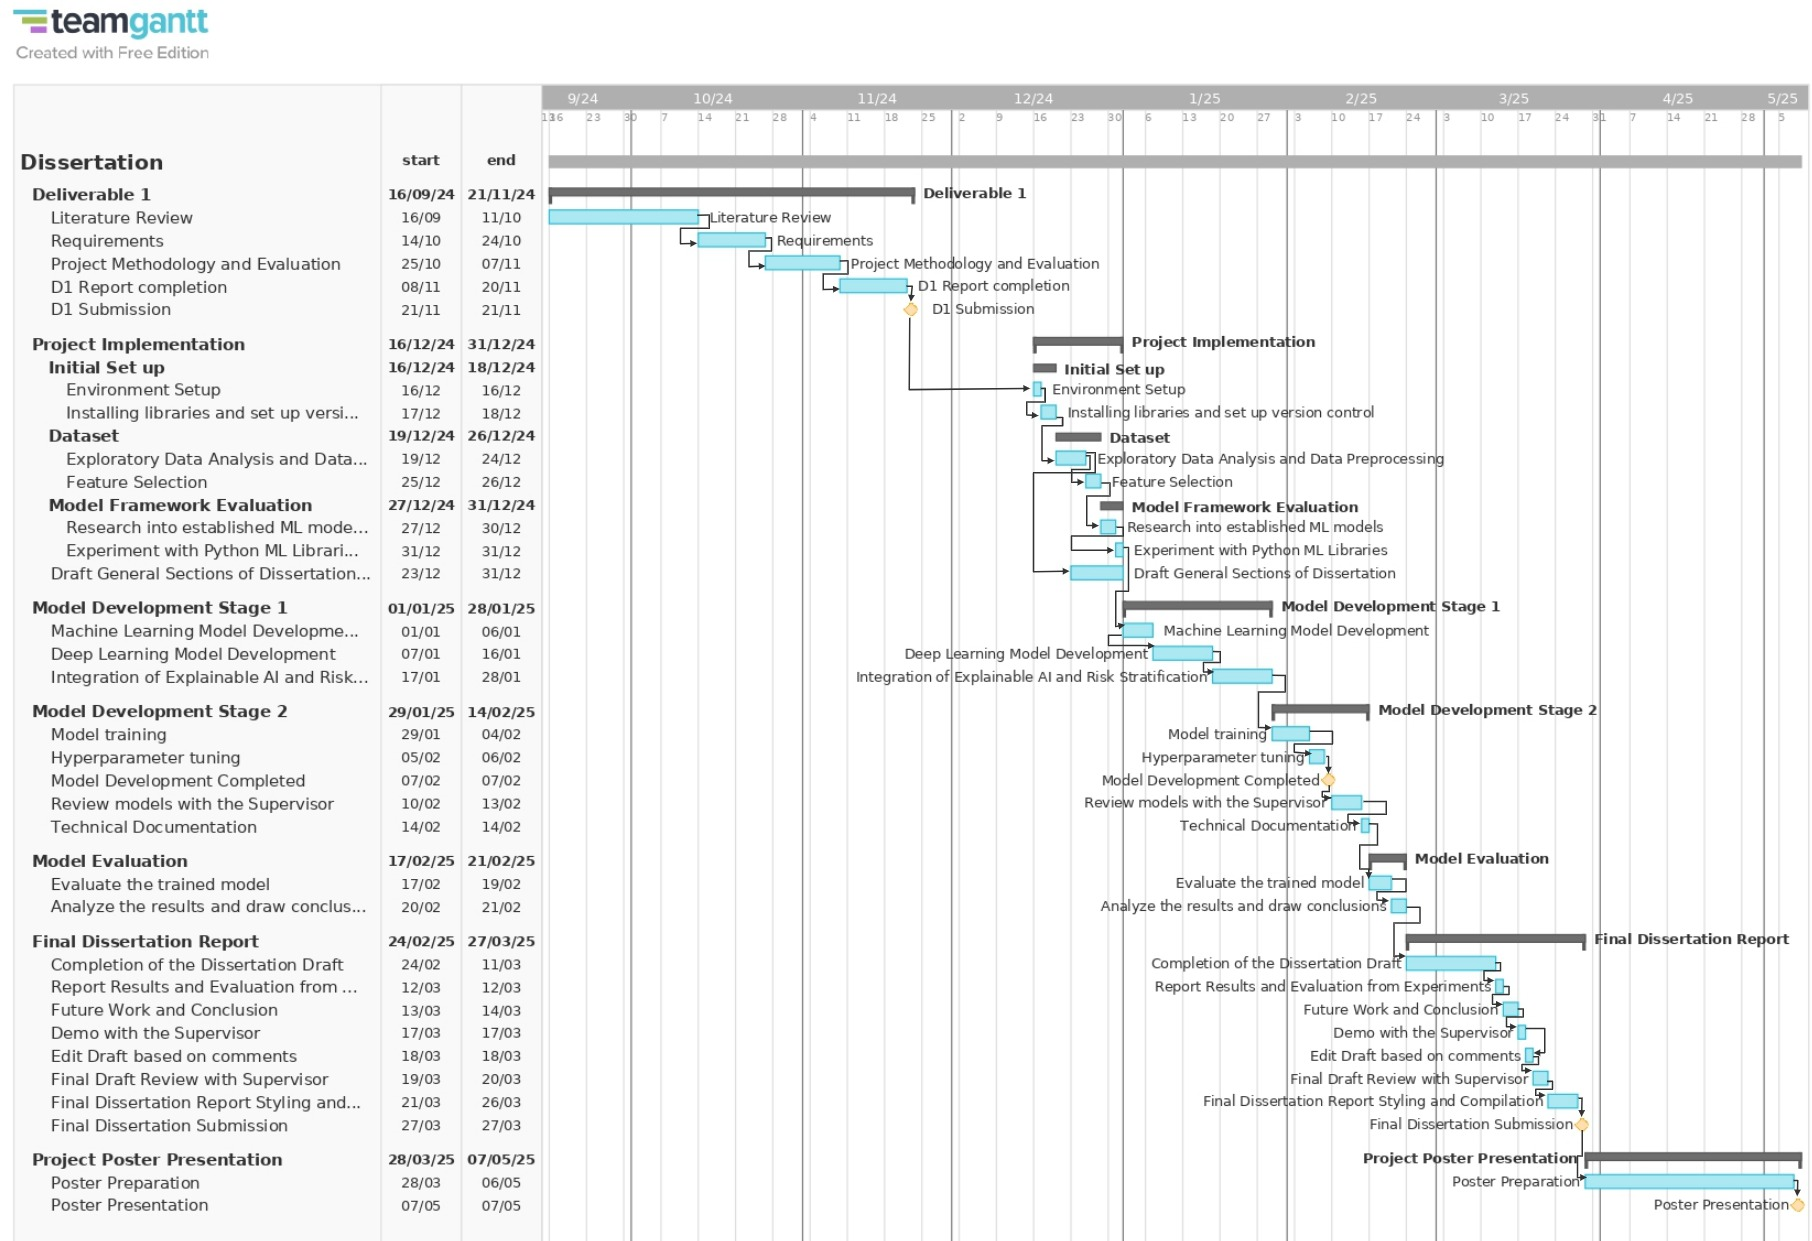
\includegraphics[width=\textwidth]{appendices/images/Dependency_GanttChart.jpg}
    \caption{Gantt Chart showing the project timeline}
    \label{fig:Gantt Chart}
\end{figure}


\vspace{0.5 cm}
\subsection{Risk Management}\leavevmode
\\Risk analysis is an important component of project management. It involves identifying potential risks, assessing their impact, and strategically developing techniques to mitigate or eliminate the risks.
Risk management is essential for ensuring project success, especially in sensitive fields like disease prediction in the healthcare sector. 
\\
The following table presents the risk analysis for this project. Each identified risk is assigned a unique risk ID and classified by type, depending on whether it pertains to people, tools, or project requirements. Risks are further categorized based on their likelihood of occurrence and impact on the project, with high, medium, and low priority levels. Additionally, an action type and an action plan have been planned for managing any issues that may arise during the development process. 
\vspace{0.5 cm}
The priority of each risk is colour-coded for the reader's clarity:

\begin{itemize}
    \item \textbf{\textcolor{red}{High Priority risks}}: Risks that need immediate action.
    \item \textbf{\textcolor{orange}{Medium Priority risks}}: Risks that need to be addressed but are less critical than high-priority risks.
    \item \textbf{\textcolor{green}{Low Priority risks}}: Risks that have a lower likelihood of occurrence or impact but should still be monitored.
\end{itemize}
\vspace{0.5 cm}
\\

% Define colors
\definecolor{riskred}{RGB}{255, 102, 102}     % Light red for R1-R5
\definecolor{riskorange}{RGB}{255, 178, 102}  % Light orange for R6-R7
\definecolor{riskgreen}{RGB}{102, 255, 102}   % Light green for R8

\begin{longtable}{|p{0.8cm}|p{2.3cm}|p{2cm}|p{1.8cm}|p{1.4cm}|>{\centering\arraybackslash}p{2cm}|p{5cm}|}
\hline
\textbf{Risk ID} & \textbf{Risk} & \textbf{Type} & \textbf{Likelihood} & \textbf{Impact} & \textbf{Action} & \textbf{Action Plan} \\
\hline
\endfirsthead
\hline
\textbf{Risk ID} & \textbf{Risk} & \textbf{Type} & \textbf{Likelihood} & \textbf{Impact} & \textbf{Action} & \textbf{Action Plan} \\
\hline
\endhead
\hline
\endfoot
\hline
\endlastfoot

\cellcolor{riskred} R1 & Data Accessibility & Requirements & Low & Medium & Mitigate & Use alternate datasets proposed in other research papers. \\
\hline
\cellcolor{riskred} R2 & Model Complexity & Requirements & Medium & High & Eliminate & Research necessary skills and topics before feature implementation and begin promptly. \\
\hline
\cellcolor{riskred} R3 & Poor Model Performance & Requirements & Medium & Low & Recognize & Investigations into suboptimal performance will be conducted, with findings documented for field advancement. The technique will be refined to improve effectiveness. \\
\hline
\cellcolor{riskred} R4 & Development Tools and Limitations in Computational Resources & Tools & High & Medium & Eliminate & Secure more powerful computational resources beforehand or resort to services/platform like Google Collab. Use alternate tools. \\
\hline
\cellcolor{riskred} R5 & Project Scheduling & Time & Medium & High & Eliminate & Allow sufficient time and allocate resources for tasks expected to be more time-consuming in the planned schedule. \\
\hline
\cellcolor{riskorange} R6 & Supervisor Availability & People & Medium & Medium & Recognize & Regular check-ins with the supervisor, with contingency plans if supervisor availability is limited. \\
\hline
\cellcolor{riskorange} R7 & Student Health & People & Low & Medium & Recognize & Prioritize personal health and ensure work-life balance to maintain productivity. Plan for breaks if needed. \\
\hline
\cellcolor{riskgreen} R8 & SHAP Implementation Complexity & Requirements & Medium & High & Eliminate & Plan time for SHAP testing, use documentation and refer to similar case studies to address implementation challenges early. Allocate extra time for SHAP setup. 
\hline
\caption{Risk Analysis} 
\end{longtable}

\vspace{0.2 cm}
A risk matrix plotting each risk ID against its likelihood and impact is presented below.
\vspace{-0.4 cm}
\begin{figure}[H]
    \centering
    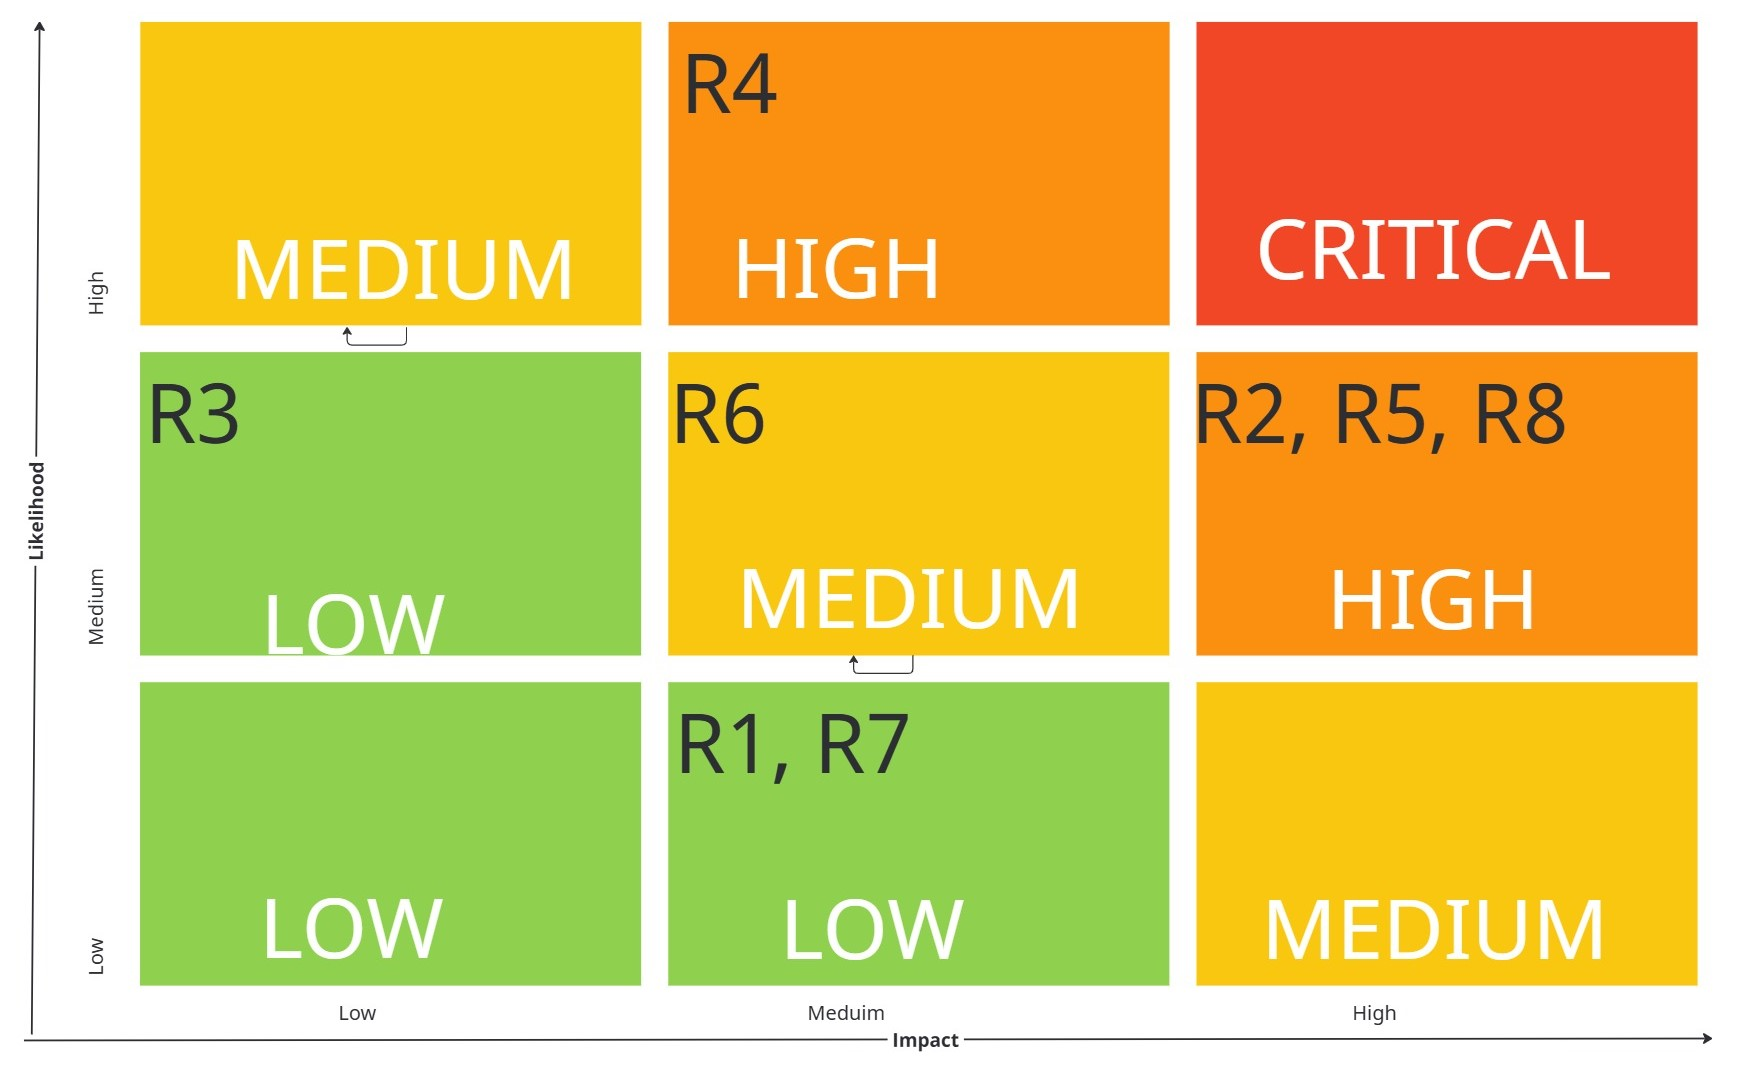
\includegraphics[width=400px]{appendices/images/Risk Matrix Template.jpg}
    \caption{Risk Matrix }
    \label{fig:Risk Matrix }
\end{figure}
\label{tab:risk_analysis}
